\chapter{Destructive 3D phenotyping pipeline}

\section{Introduction}

Estimating the plant phenotypes accurately and efficiently can help to bridge the gap between genotype and phenotype. The traditional phenotyping measurement is time-consuming, laborious, and often not accurate. Although several authors have developed 2D image-based phenotyping methods which are more efficient, non-destructive, and have higher throughput \citep{yang_greenness_2015,guo_easypcc_2017,zou_broccoli_2019}, these approaches are unable to describe the plant 3D structure due to the occlusion and dimension loss when projecting onto the 2D plane. As a result, it produces inaccuracies and uncertainties for advanced phenotyping applications.

To overcome the drawbacks of 2D image-based phenotyping, several studies have paid attention to 3D approaches. \citet{paulus_measuring_2019} and \citet{kochi_introduction_2021} have summarized the current approaches to obtain 3D plant models; and a large number of studies have chosen the 3D reconstruction by photogrammetry using common RGB cameras due to the low device cost \citep{xiao_estimating_2021,zermas_3d_2020,zhang_estimating_2016}. The 3D model of an object can be calculated from images from different view angles with enough overlap (Fig.~\ref{fig:des1}). The full process includes structure-from-motion (SfM, to calculate relative positions between images and the rough 3D point cloud of the object), multi-view stereo (MVS, to densify the 3D point cloud of the object), and surface reconstruction (to obtain object 3D mesh model); for more details, please refer to this book \citep{hartley_multiple_2000} and this review \citep{snavely_scene_2010}. Although the proposed 3D image-based phenotyping was proved feasible for many agriculture applications, when apply to the broccoli head cases, the current 3D method is facing several challenges.

\begin{figure}[htb]
  \begin{center}
    \resizebox{\textwidth}{!}{
      \includegraphics{figures/des/sfm_types.pdf}
    }
  \end{center}
  \caption[Current photogrammetry (3D reconstruction) methods]{
    The current camera placement for 3D reconstruction. (a) fixing the object and taking images using multiple fixed cameras at the same time, also called forward intersection; (b) fixing the object but taking images by using a moved camera, also called backward resection; (c) rotating the object and taking images using fewer multiple fixed cameras, or a camera fixed at different locations for each rotation.
  }
  \label{fig:des1}
\end{figure}

The first challenge is image acquisition for cost-effective reconstruction. Several authors used the following three approaches to acquire images (Fig.~\ref{fig:des1}): (a) fix the object and fix cameras \citep{nguyen_structured_2015}; (b) fix the object and move a camera manually \citep{xiao_image-based_2020} or using robotic arms \citep{cao_quantifying_2019,nguyen_3d_2016}; and (c) rotate the object and fix or move the camera(s) \citep{kochi_3d_2018,gao_novel_2021}. The main drawback of these imaging approaches is that it is difficult to provide fully complete view angles of plants within acceptable cost. Most methods can only capture images of the sunny side (such as the front surface of leaves and the top of broccoli crowns), while capturing images of the shaded side (such as the back surface of leaves and the downside of broccoli crowns) is more difficult and requires extreme upward viewing angles (Fig.~\ref{fig:des1}.d). Even if such images can be acquired, they often fail to align with the 3D model due to insufficient feature matching points. Hence, a solution is required to improve the integrity of the reconstructed plant 3D model, especially for the solid closed harvestable organs like broccoli head.

The second challenge is image preprocessing for the acquired images. Compared to the approach of building the full scenario, segmenting the plant parts out \citep{ge_method_2019}, and denoising \citep{wu_mvs-pheno_2020}; some studies segmented and masked the foreground (plant) area before doing the 3D reconstruction \citep{nguyen_3d_2016,kochi_3d_2018}, to improve the model quality and eliminate the effect of background noises. Although the controlled environment can provide pure background and stable lighting, it is still challenging to develop a robust algorithm to segment the broccoli area perfectly, especially to handle the shadows caused by the irregular broccoli head shape at the different growing stages. Some outdoor studies showed the power of deep learning for plant area detection and segmentation \citep{zhou_monitoring_2020,blok_effect_2021,garcia_towards_2021}, but limited by the GPU memory, the original images often resized to smaller sizes for deep learning. For example, \citet{zhou_monitoring_2020} resized to $1440 \times 1080$, \citet{blok_effect_2021} resized to $1024 \times 1024$, and \citet{garcia_towards_2021} resized to $640 \times 480$. The plant mask produced in such a resolution can not fit well into the original images in detail (in our case, is $5184 \times 3456$), and hence also need a method to produce detailed masks with the original resolution.

In this study, we applied several strategies to overcome the previously mentioned challenges and provide a labor-saving pipeline for obtaining high-quality 3D models for destructive broccoli heads. The objectives of this study were to: (1) develop the dual-rotation object strategy with a fixed camera to collect images with abundant view angles for integrity 3D reconstruction; (2) implement the two-step deep learning workflow to acquire the detailed plant masks on the original images; (3) calculate the 3D morphological traits of broccoli head and crown; and (4) validate the estimated head size using the manual measurements. This pipeline also has great potential to be applied to other solid closed harvestable organs, such as potatoes, cauliflowers, and sweet potatoes, which are related to the profit directly. Meanwhile, using just a simple RGB camera and several low-cost commercial photographic equipments, makes it easier to be widely-spread use.


\section{Methods and Materials}

\subsection{Plant 3D model acquisition}

% plant materials, the information for fields and selective sampling

\subsubsection{Imaging device}

% figure2: 3D reconstruction devices
\begin{figure}[htb]
  \begin{center}
    \resizebox{\textwidth}{!}{
      \includegraphics{figures/des/img_recons.pdf}
    }
  \end{center}
  \caption[The plant 3D model reconstruction workflow]{
    The Plant 3D model reconstruction workflow; (a) devices for taking plant images, with a marker plane used as scalebar references; (b) an automatic horizontal rotating platform, which can rotate at a given angle and then stop for a short interval for image taking. The vertical rotation of plants (flip) requires manual operation; (c) different photographic perspectives images taken by the infrared signal auto-imaging system; (d) partial marker detection to avoid misleading image alignment, where only markers on one rotating image group (orange) are detected and not on the others (blue); (e) plant part segmentation using deep learning; (f) the final 3D plant model produced by Metashape; and (g) the scripts for batch processing a large number of plants.
  }
  \label{fig:des_img_recons}
\end{figure}

\subsubsection{Image preprocessing}



\subsubsection{Batch 3D reconstruction}

% marker detection for one round and ignore for others

% the batch preprocessing 

\subsection{Phenotypic traits extraction}

% figure3: general workflow
\begin{figure}[htbp!]
  \begin{center}
    \resizebox{0.9\textwidth}{!}{
      \includegraphics{figures/des/seg_algorithm.pdf}
    }
  \end{center}
  \caption[The algorithms for plant 3D model analysis]{
    The algorithms for plant 3D model analysis; (a) crown segmentation, to split the broccoli crown part and the stem part; (b) direction correction, to rotate the broccoli vertically to the z-axis positive direction; and (c) traits calculation.
  }
  \label{fig:des_seg_alg}
\end{figure}

\subsubsection{Head segmentation}

\subsubsection{Upward direction correction}

\subsubsection{Traits calculation}


\subsection{Validation}

% field measurmenet

% r2 and rmse


\section{Results}

\subsection{Image preprocessing}

% figure4: unet + casadePSP results
% add more examples
\begin{figure}[htbp!]
  \begin{center}
    \resizebox{\textwidth}{!}{
      \includegraphics{figures/des/dl_seg.pdf}
    }
  \end{center}
  \caption[Two deep learning segmentation results]{
    Examples of two deep learning segmentation results. (a) is the original image of the broccoli head, the resolution is $5184 \times 3456$ pixel; (b) is the output of the UNet segmentation, the resolution is $256 \times 256$ pixel, which is not enough as final plant masks; and (c) the output of the refined high-resolution mask using CasadePSP based on the UNet output. The mask has the same resolution as the original image.
  }
  \label{fig:des_dl_seg}
\end{figure}

\subsection{Plant 3D model}

% figure5: comparison between real photo and photos + model 3 views
\begin{figure}[htb]
  \begin{center}
    \resizebox{\textwidth}{!}{
      \includegraphics{figures/des/model_results.pdf}
    }
  \end{center}
  \caption[The obtained 3D models]{
    Some examples of obtained 3D models. (a) the image of 15 broccoli heads in the real world; (b) the obtained 3D models of corresponding broccoli heads; and (c) the different views of one broccoli head 3D model.
  }
  \label{fig:des_model_results}
\end{figure}

\subsection{Traits extraction}

% figure6: head extraction
% change to all reulst + one demo
\begin{figure*}[htb]
  \centering
  \begin{subfigure}[b]{0.475\textwidth}
    \centering
    \includegraphics[width=\textwidth]{figures/des/7-2-2.png}
    \caption{ID 7-2-2}
  \end{subfigure}%
  \hfill
  \begin{subfigure}[b]{0.475\textwidth}
    \centering
    \includegraphics[width=\textwidth]{figures/des/1-5.png}
    \caption{ID 1-5}
  \end{subfigure}
  \vskip\baselineskip

  \begin{subfigure}[b]{0.475\textwidth}
    \centering
    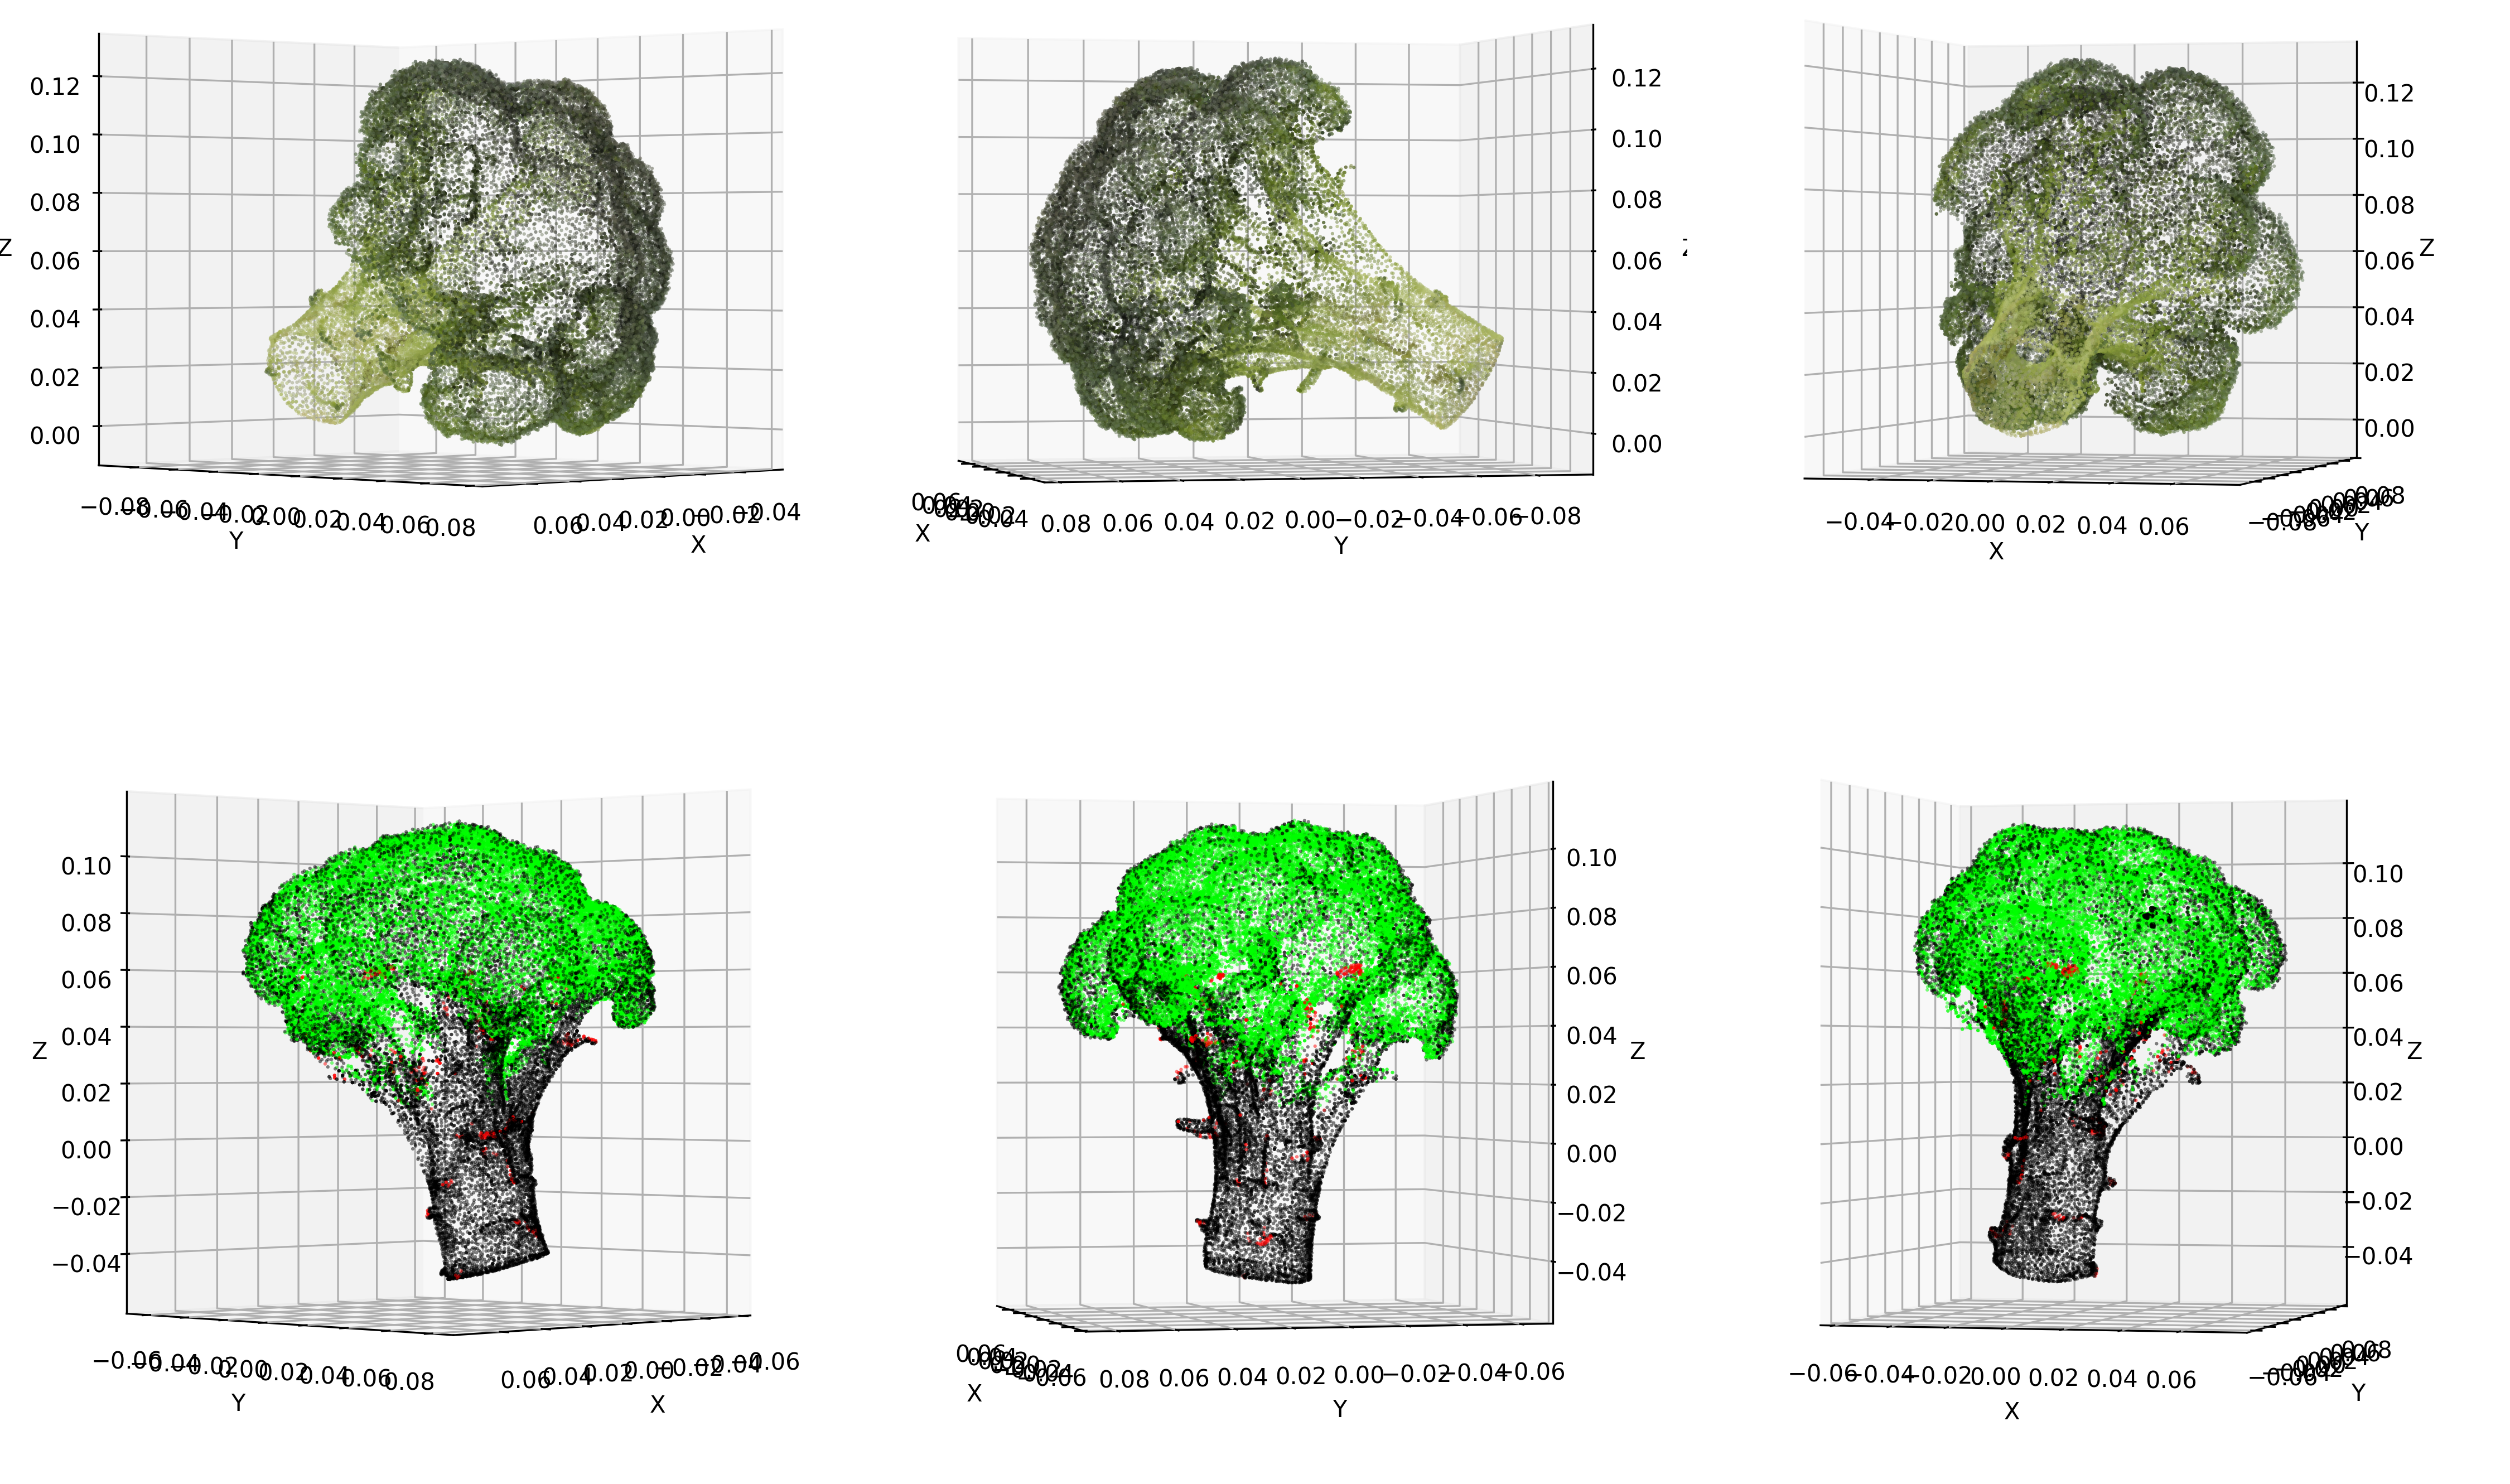
\includegraphics[width=\textwidth]{figures/des/2-23.png}
    \caption{ID 2-23}
  \end{subfigure}%
  \hfill
  \begin{subfigure}[b]{0.475\textwidth}
    \centering
    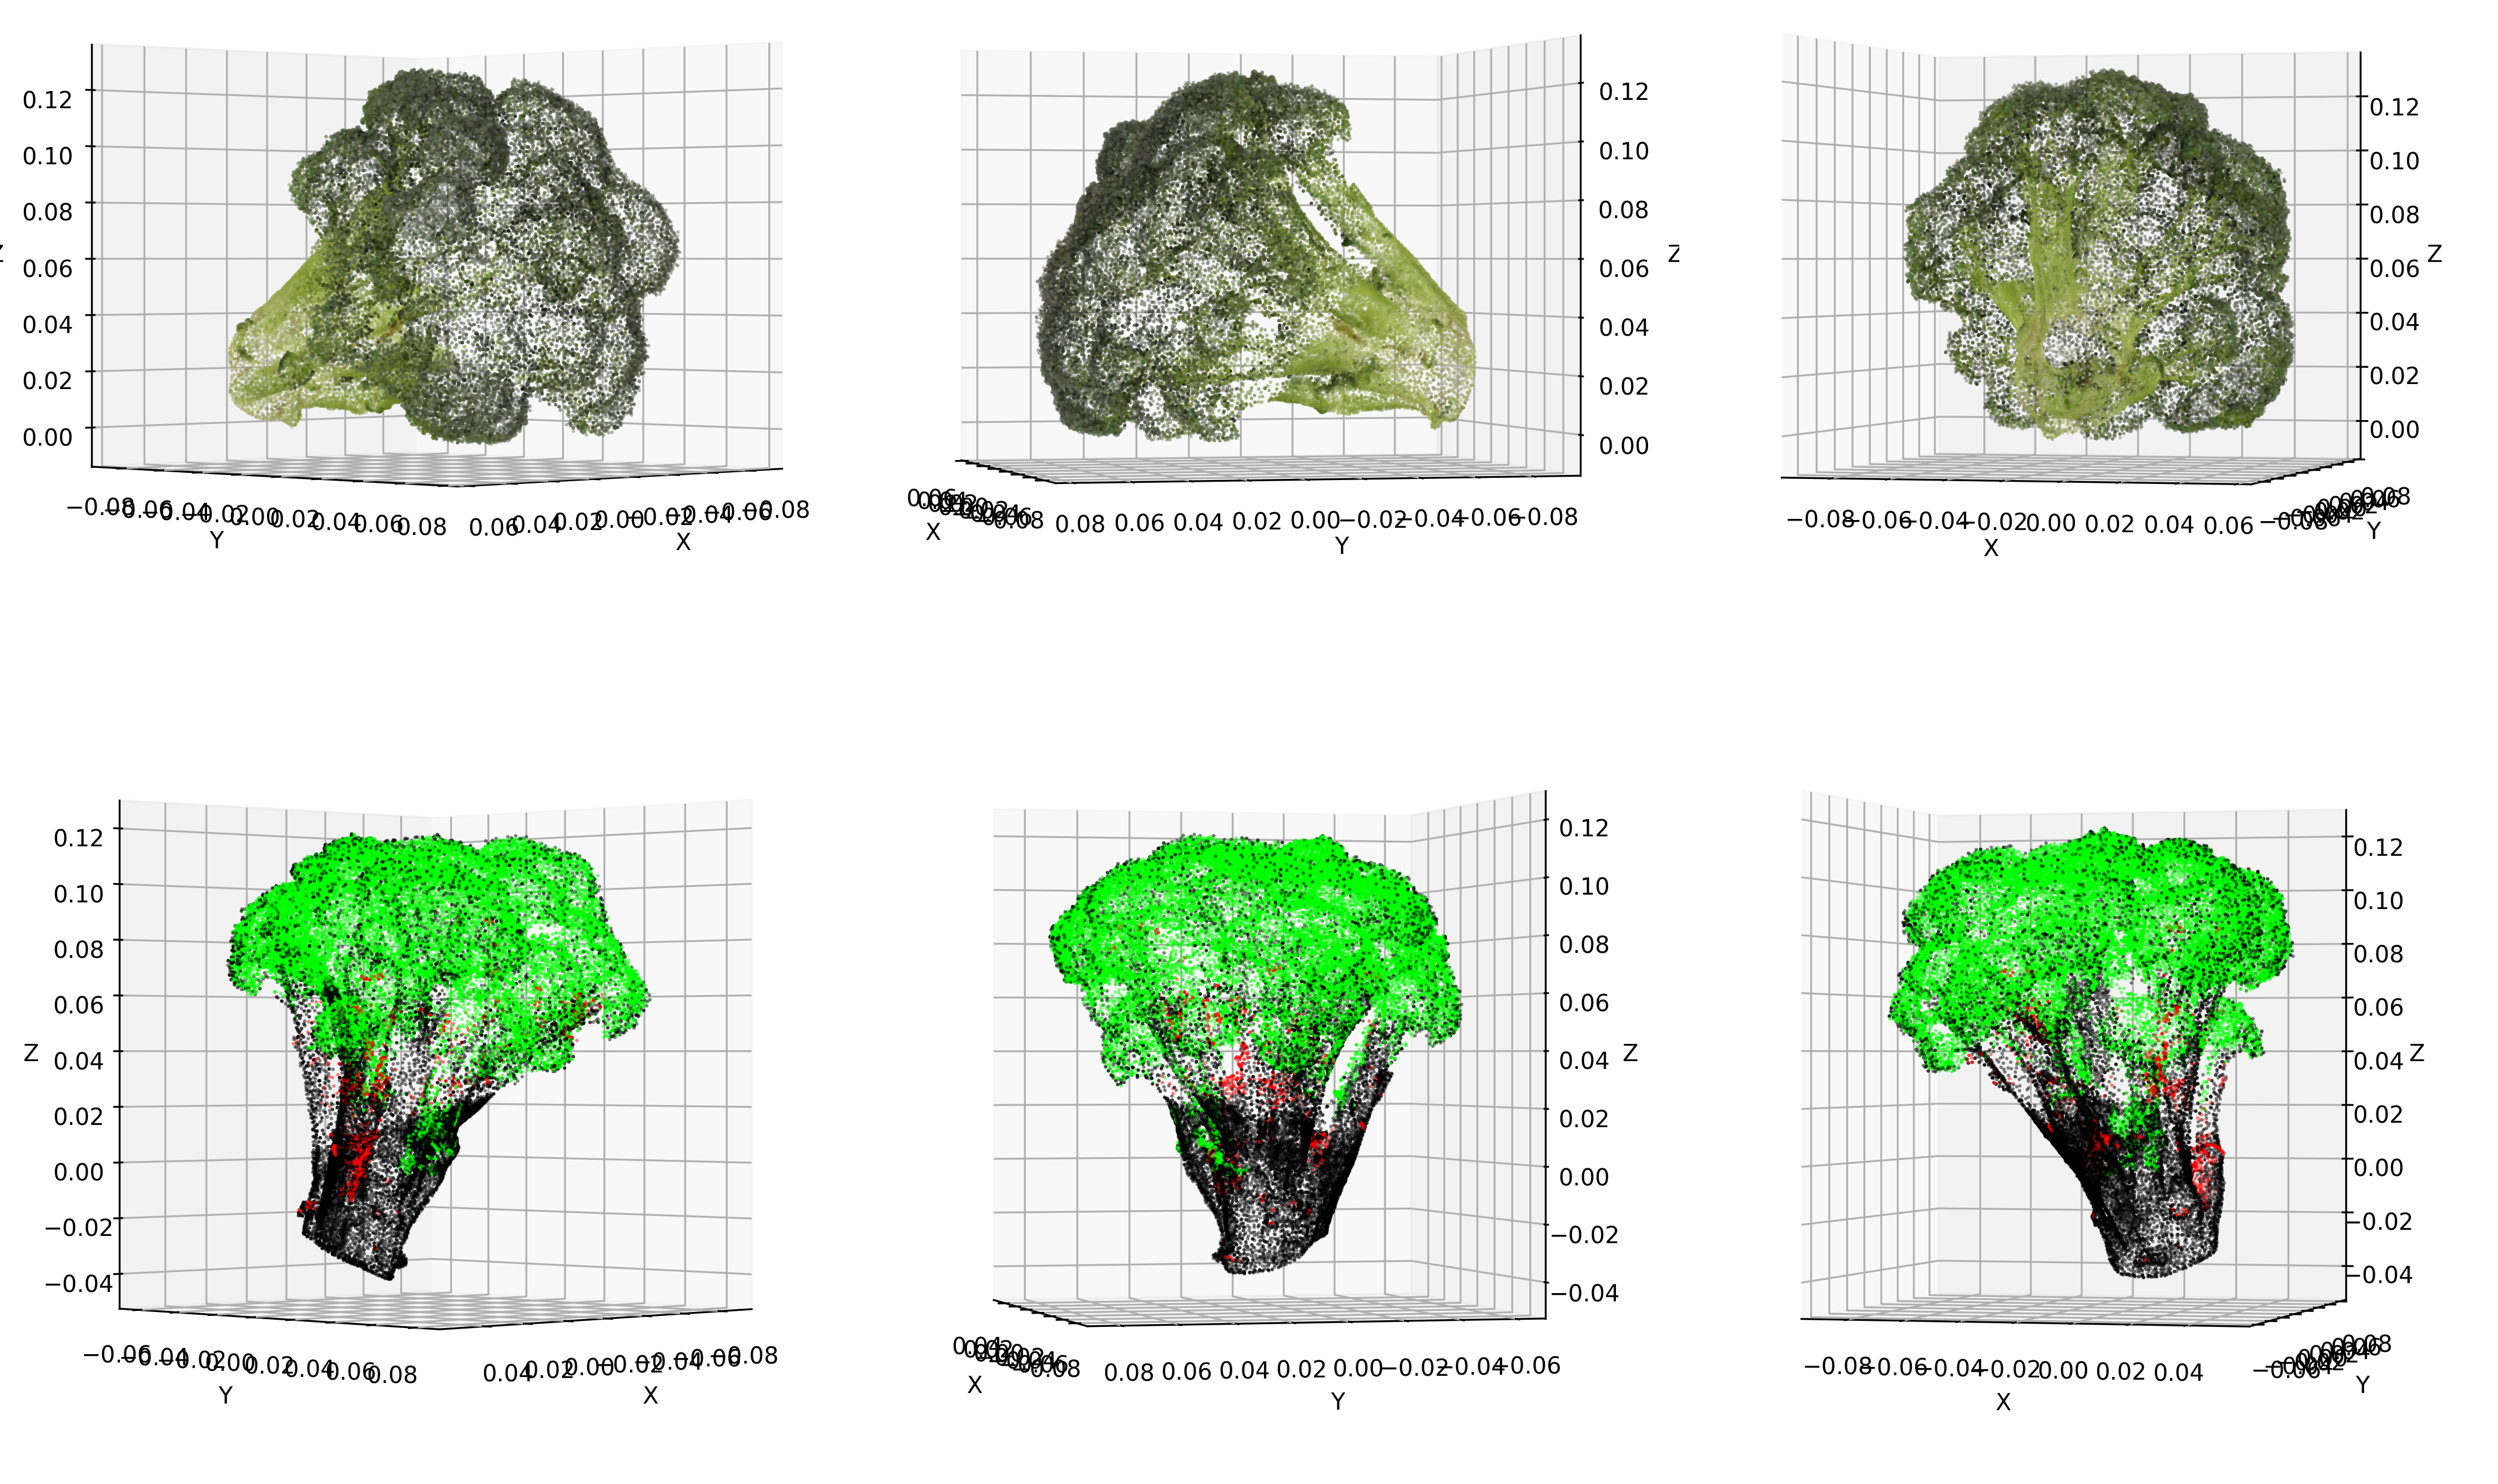
\includegraphics[width=\textwidth]{figures/des/1-33.png}
    \caption{ID 1-33}
  \end{subfigure}%
  \caption[Examples of plant 3D model analysis at different growing stages]{
    Examples of plant 3D model analysis at different growing stages. The upper parts are the original coordinates of the obtained 3D models, while the lower parts are the segmented and direction-corrected results, the red parts are removed noises. Three columns show the corresponding azimuth angle views at $45^\circ$, $165^\circ$, and $285^\circ$ for the same 3D model.
  }
  \label{fig:des6}
\end{figure*}


\subsection{Validation}

\begin{figure}[htb!]
  \begin{center}
    \resizebox{\textwidth}{!}{
      \includegraphics{figures/des/method_compare.pdf}
    }
  \end{center}
  \caption[The comparison between the proposed phenotyping pipeline and manual measurement]{
    The comparison between the proposed phenotyping pipeline and manual measurement. The shortest length and longest length of the broccoli head are compared. For the proposed pipeline, it uses two methods to estimate those lengths. One is using the length and width of the minimum bounding rectangle, the other is using the major and minor axes of the fitted ellipse.
  }
  \label{fig:des_compare}
\end{figure}

\section{Discussion}



\section{Conclusion}